\documentclass[letterpaper]{article}
\usepackage{aaai}
\usepackage{times}
\usepackage{helvet}
\usepackage{courier}
\usepackage{amsmath,amssymb,amsthm,fullpage,mathtools}
\usepackage{mathtools}
\usepackage[english]{babel}
\usepackage{graphicx}
\usepackage{fontspec}
\usepackage{newunicodechar}
\usepackage{multicol}
\usepackage[margin={1.5cm,1.5cm}]{geometry}
\usepackage{hyperref}
\DeclareMathOperator*{\argmax}{\arg\!\max}
\setlength{\pdfpagewidth}{8.5in}
\setlength{\pdfpageheight}{11in}

\usepackage{tikz} % for dependency graph
\usepackage{listings} % to include code


% \pdfinfo{
% /Title (Classifying Malicious Software)
% /Author (Kevin K. Eskici, Luis A. Perez, Aidi Zhang)}
\setcounter{secnumdepth}{0}

% we want to adjust the seperationg between columns
\setlength{\columnsep}{1cm}

\title{Practical 2: Classifying Malicious Software}
\author{Kevin Eskici\thanks{keskici@college.harvard.edu}, Luis A. Perez\thanks{luisperez@college.harvard.edu}, Aidi Zhang\thanks{aidizhang@college.harvard.edu} \\
Kaggle Team: cacheMoney \\
Computer Science, Harvard University}

\date{\today} 

\begin{document}

\maketitle

\begin{abstract}
\begin{quote}
In this paper, we empirically tackle the problem of classifying malicious programs based on a trace of their execution history. Specifically, given a training set of 3086 XML files, we attempt to learn a total of 15 different malware classifications, and test our results on 3724 XML files (our testing set). We explore in-depth both simple generative models using Gaussian priors as well as more complex and (we find) effective models such as Random Forests. We deviate to explore other possible machine learning methods, such as SVNs and KNN. Additionally, we explore three classes of features: (1) simple count based features, (2) action based features such as server requests, and (3) structural program features such as n-grams. We find that while somewhat helpful, more of the above features typically leads to over-fitting of data and to little improvement in our random forest model. In conclusion, a random forest model with features from each of the three aforementioned categories performed the best, both locally (achieving >90\% accuracy on cross-validation), publicly (achieving >83\% accuracy), and privately (achieving > 82\% accuracy).  
\end{quote}
\end{abstract}

\section{Introduction}

\noindent Classification is typically a difficult problem to solve, especially in the general case where the problem involves classifying $n$ items into $k > 2$ distinct classes. For the binary case of $k=2$, multiple approaches exists which have been shown to be efficient, such as logistic regression, a class-conditional generative classifier, Fisher's discriminant approach \footnote{\href{http://research.cs.tamu.edu/prism/lectures/pr/pr_l10.pdf}{Linear discriminant analysis}}, neural networks, support vector machines, etc. Many of these models generalize relatively easily to multiple classes, but some, like Fisher's discriminant, require more effort to generalize. \\

\noindent In this paper, we discuss a specific instance of the class of classification problem. In particular, we explore the problem of classifying execution traces of programs on a Windows machine, given in XML format, into 14 distinct viral class, shown in Figure \ref{tab:virus_classes}. The table also shows the distribution of each viral type in both the test data and the training data, as originally reported. Throughout the paper, we fill in some gaps in the table. The total number of training executable files was 3086, and the total number of unknown executable files was 3724.\\

\noindent Due to the the fact that our problem was more general than $k = 2$, we used the algorithms that could easily be generalized. Our first attempt focused on a simple use of a generative classifier using the sample means and sample covariance matrices. We opted to skip the logistic regression on basic features due to the fact it allows only for linear decision boundaries in the features space and we expected our data to be highly non-linear in the feature space, given the variability in virus types \footnote{\href{http://www.omnisecu.com/security/types-of-computer-viruses.php}{Types of Windows OS Viruses}}. Previous experience also indicated better performance for the simple generative model \footnote{In particular, Problem 4 from Homework 2: Linear Classification}. However, the generative model proved to be rather inadequate for our particular malware classification problem. After tweaking it for optimal performance, we moved on to using a Random Forest Classifier and k-nearest neighbors (KNN), two methods we hoped would improve the accuracy of our prediction. In conclusion, we managed to correctly match approximately $90.02\%$ of the data, according to our cross-validation tests, and a we managed an accuracy of approximately $83.14\%$ on our public test data, according to the Kaggle site.\\
 
% Information on the virus classification parameters for our training data as well as our test data
\noindent Considering the optimal public accuracy score was approximately $83.14\%$, we were comfortable with our results. Therefore, we now describe our methods.

\section{Methodology}
We attempted multiple different models to achieve our final optimal solution: KNN, Random Forest, SVNs, and a simple generative approach. In addition to the models attempted above, we also extracted features from the provided XML files using the sample ElementTree\footnote{\href{https://docs.python.org/3/library/xml.etree.elementtree.html}{Python ElementTree Library}} structure. We tried a few different approaches, but at the end of the day, we settled on extracting three key pieces of information - number of system calls, number of calls made to each system function, and number of sequences of calls, typically known in literature as n-grams. We also attempted a bag-of-words approach to the XML file feature extraction, which failed spectacularly for most of our models.

% Generative Approach
\subsection{Generative Model}
The generative model is simple to implement yet relatively effective. It has a closed form solutions, which was calculated in Bishop, and contains no hyper-parameters, thereby removing the need for parameter optimization. Theoretically, it could be possible to optimize the initial assumption of a Gaussian prior using information about the testing set. However, after extended research, we determined that the files in our testing set differed significantly from our training set. As shown in Figure \ref{tab:virus_classes}, the distribution of ``None'' labels is lower by a factor of approximately $25\%$. The feature that indicated the largest difference, however, is highlighted by Figure \ref{fig:file_size} which shows that the test files tend to be twice as large as the files in the training set. Therefore, we resolved to simple attempt the generative model. \\

\begin{figure}
	\centering
	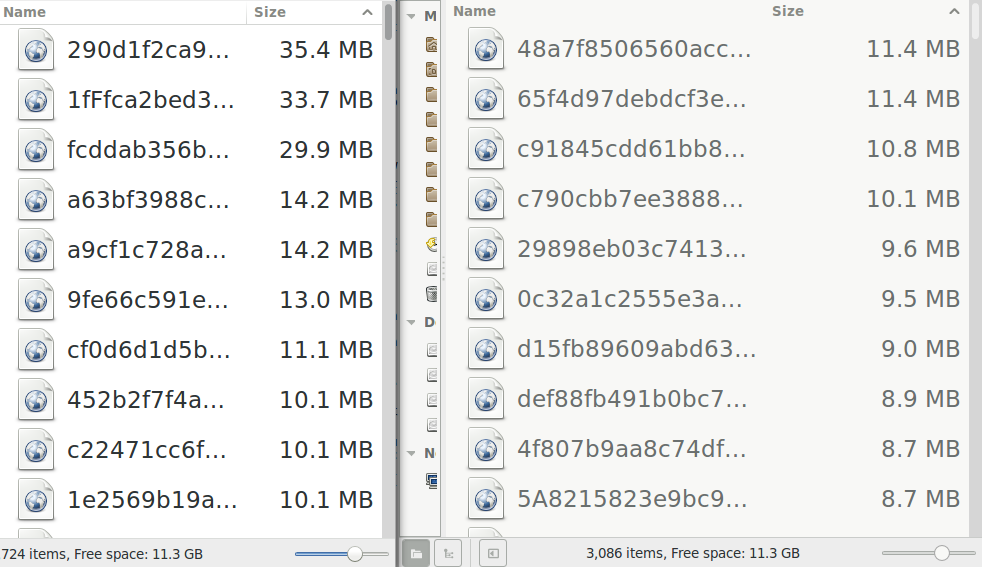
\includegraphics[scale=0.2]{file_size}
    \caption{Testing and Training Data Sets, sorted by size in the file-viewer. We note that the testing files appear to be significantly larger than the training set files. This difference discouraged us from attempting to over-optimize based on the training data. We wanted to generalize our learning, not over-fit our training set.}
    \label{fig:file_size}
\end{figure}

\noindent First, let $C_k$ be the $k$-th class. In our case, we have $k = 15$. Then we let the set $\{\vec{x}_n, t_n \}_{n=1}^N$ be our supervised training set. For the generative model, what we're attempting to calculate is the probability of a class given a data-point. For simplicity, we assume that the distribution is Gaussian. The above assumptions lead us to the below result, where $D$ is the number of features per datum:  
\begin{align}
    \mathbb{P}(C_k \mid \vec{x}) &= \mathcal{N}(\vec{\mu_k^*}, \Sigma_k^*) \\
    =& \frac{|\Sigma^{-\frac{1}{2}}|}{(2\pi)^{D/2}}e^{-\frac{1}{2}(\vec{x_k} - \vec{\mu_k^*})^T \Sigma^*(\vec{x} - \vec{\mu_k^*})}
\end{align}

\noindent Following the derivation in Bishop, however now without the assumption that each class shares the same covariance matrix, we know that the optimal value for $\vec{\mu*}$ is given by the following, where we sum over the elements in class $k$ and divide by $N_k$, the total number of elements in that class:
\begin{align}
	\vec{\mu_k^*} &= \frac{1}{N_k}\sum_{k \in C_k} \vec{x_k}
\end{align}
or in other words, the average of the Gaussian is given by the sample average. Similarly, the optimal value for the covariance matrix, \textbf{$\Sigma_K^*$}, of the Gaussian is given by the sample covariance for each class. Once we have these two values calculated, we build a Gaussian distribution over our feature space. From that point, the model simply relies on, given a test point $\vec{x}$, calculating:
\begin{align}
	C_k &= \text{argmax}_{C_k} \left\{\mathbb{P}(C_k \mid \vec{x}) \right\}
\end{align}
One challenge with this model, however, occurs when the dimension of $D$ of our features space is larger than the number of datums, $N_k$, in each class. Looking at Table \ref{tab:virus_classes}, we note the following:
\begin{align*}
	N_9 = 0.68 * N = (0.0068)(3086) \approx 2
\end{align*}
This was both surprising and discouraging. However, the generative method can be adopted to handle cases where the covariance matrix does not have an inverse by simply replacing the $\Sigma^{-1}$ with the Moore-Penrose pseudo-inverse \footnote{\href{http://www.visiondummy.com/2014/04/geometric-interpretation-covariance-matrix/}{Geometric Interpretation of the Co-variance Matrix}}. One possible form is shown below:
\begin{align}
	\Sigma^{-1} &= (\Sigma^T\Sigma)^{-1}\Sigma^T 
\end{align}

\noindent The above allows us to avoid singular matrix errors when approximating the Gaussian distribution of each class. Another approach would have been to simply remove classes with a small number of data points. However, due to the discrepancy between the distribution of malware in the test data and in the training data, we decided that removing classes without more information about the distribution in the testing set could not be done in a methodological fashion and would likely only harm our prediction accuracy.\\
\\
\noindent After tweaking our features for optimal for this model, we achieved a result of 62.336\% accuracy in our predictions.

% Random Forest
\subsection{Random Forest}
Random forest classifiers are important ensemble methods that makes predictions by taking averages of several independent base models called decision trees. The random forest was a promising model because it is a powerful classifier tool that runs efficiently on large data, naturally weights features according to importance and relatively safe from the risk of over-fitting. There are two aspects of randomness that are explained below:\\
\\
The first step in a random forest algorithm - building individual decision trees - introduces randomness by subsetting features to train in each tree, which we call feature bagging. The intuition behind this is to prevent the existence of very strong predictors of the target variable to be present in many or all trees, causing them to be correlated. Decision trees are built by recursively finding splits on $L_t$ that maximizes the decrease in the generalization error:

\begin{equation}
\begin{split}
&E_L(Err(\phi_L(x))) \\
= \text{noise}&(x) + \text{bias}(x)^2 + Var(x)
\end{split}
\end{equation}
where noise$(x) = Err(\phi_B(x))$, bias$(x) = (\phi_B(x) - E_L(\phi_L(x)))^2$ and $Var(x) = E_L(E_L(\phi_L(x) - \phi_L(x))^2)$.\\
\\
This generalization error has a low bias term but suffers from a relatively high variance, which is why we need random forests to combine predictions of multiple trees into a single model, thereby controlling variance.\\
\\
We hence train multiple trees (forming a forest) on bootstrapped samples of training set in a process called tree bagging. Bootstrapping essentially means random sampling with replacement. This decreases the variance without affecting the bias of the model but also provides the extra benefit of de-correlating trees by showing them different subsets of the training set. The new generalization error of an ensemble of M randomized models $\phi_{L,\theta_m}$ becomes:

\begin{equation}
\begin{split}
&E_L(Err(\psi_{L,\theta_1,...,\theta_M(x)})) \\
= &\text{noise}(x) + \text{bias}(x)^2 + Var(x)
\end{split}
\end{equation}

\noindent where noise and bias stays exactly the same as before, but variance$(x) = \rho(x) \sigma^2_{L,\theta}(x) + \frac{1-\rho(x)}{M}\sigma^2_{L,\theta}(x)$ where $\rho(x)$ is the Pearson correlation coefficient between predictions of two trees build on the same training set.\\
\\
The above illustrates the bias-variance tradeoff - the stronger the randomization, our bias increases but it also makes it possible to decrease variance of our ensemble model.\\
\\
The number of decision trees, n-estimators, is a hyper-parameter that we were careful to optimize. We found the optimal number using cross-validation, and found that generally a larger number of trees resulted in better results, until a certain point of 1000-2000 trees after which results plateaued. This is shown in Figure \ref{fig:random_forest_optimizer}.

\begin{figure}
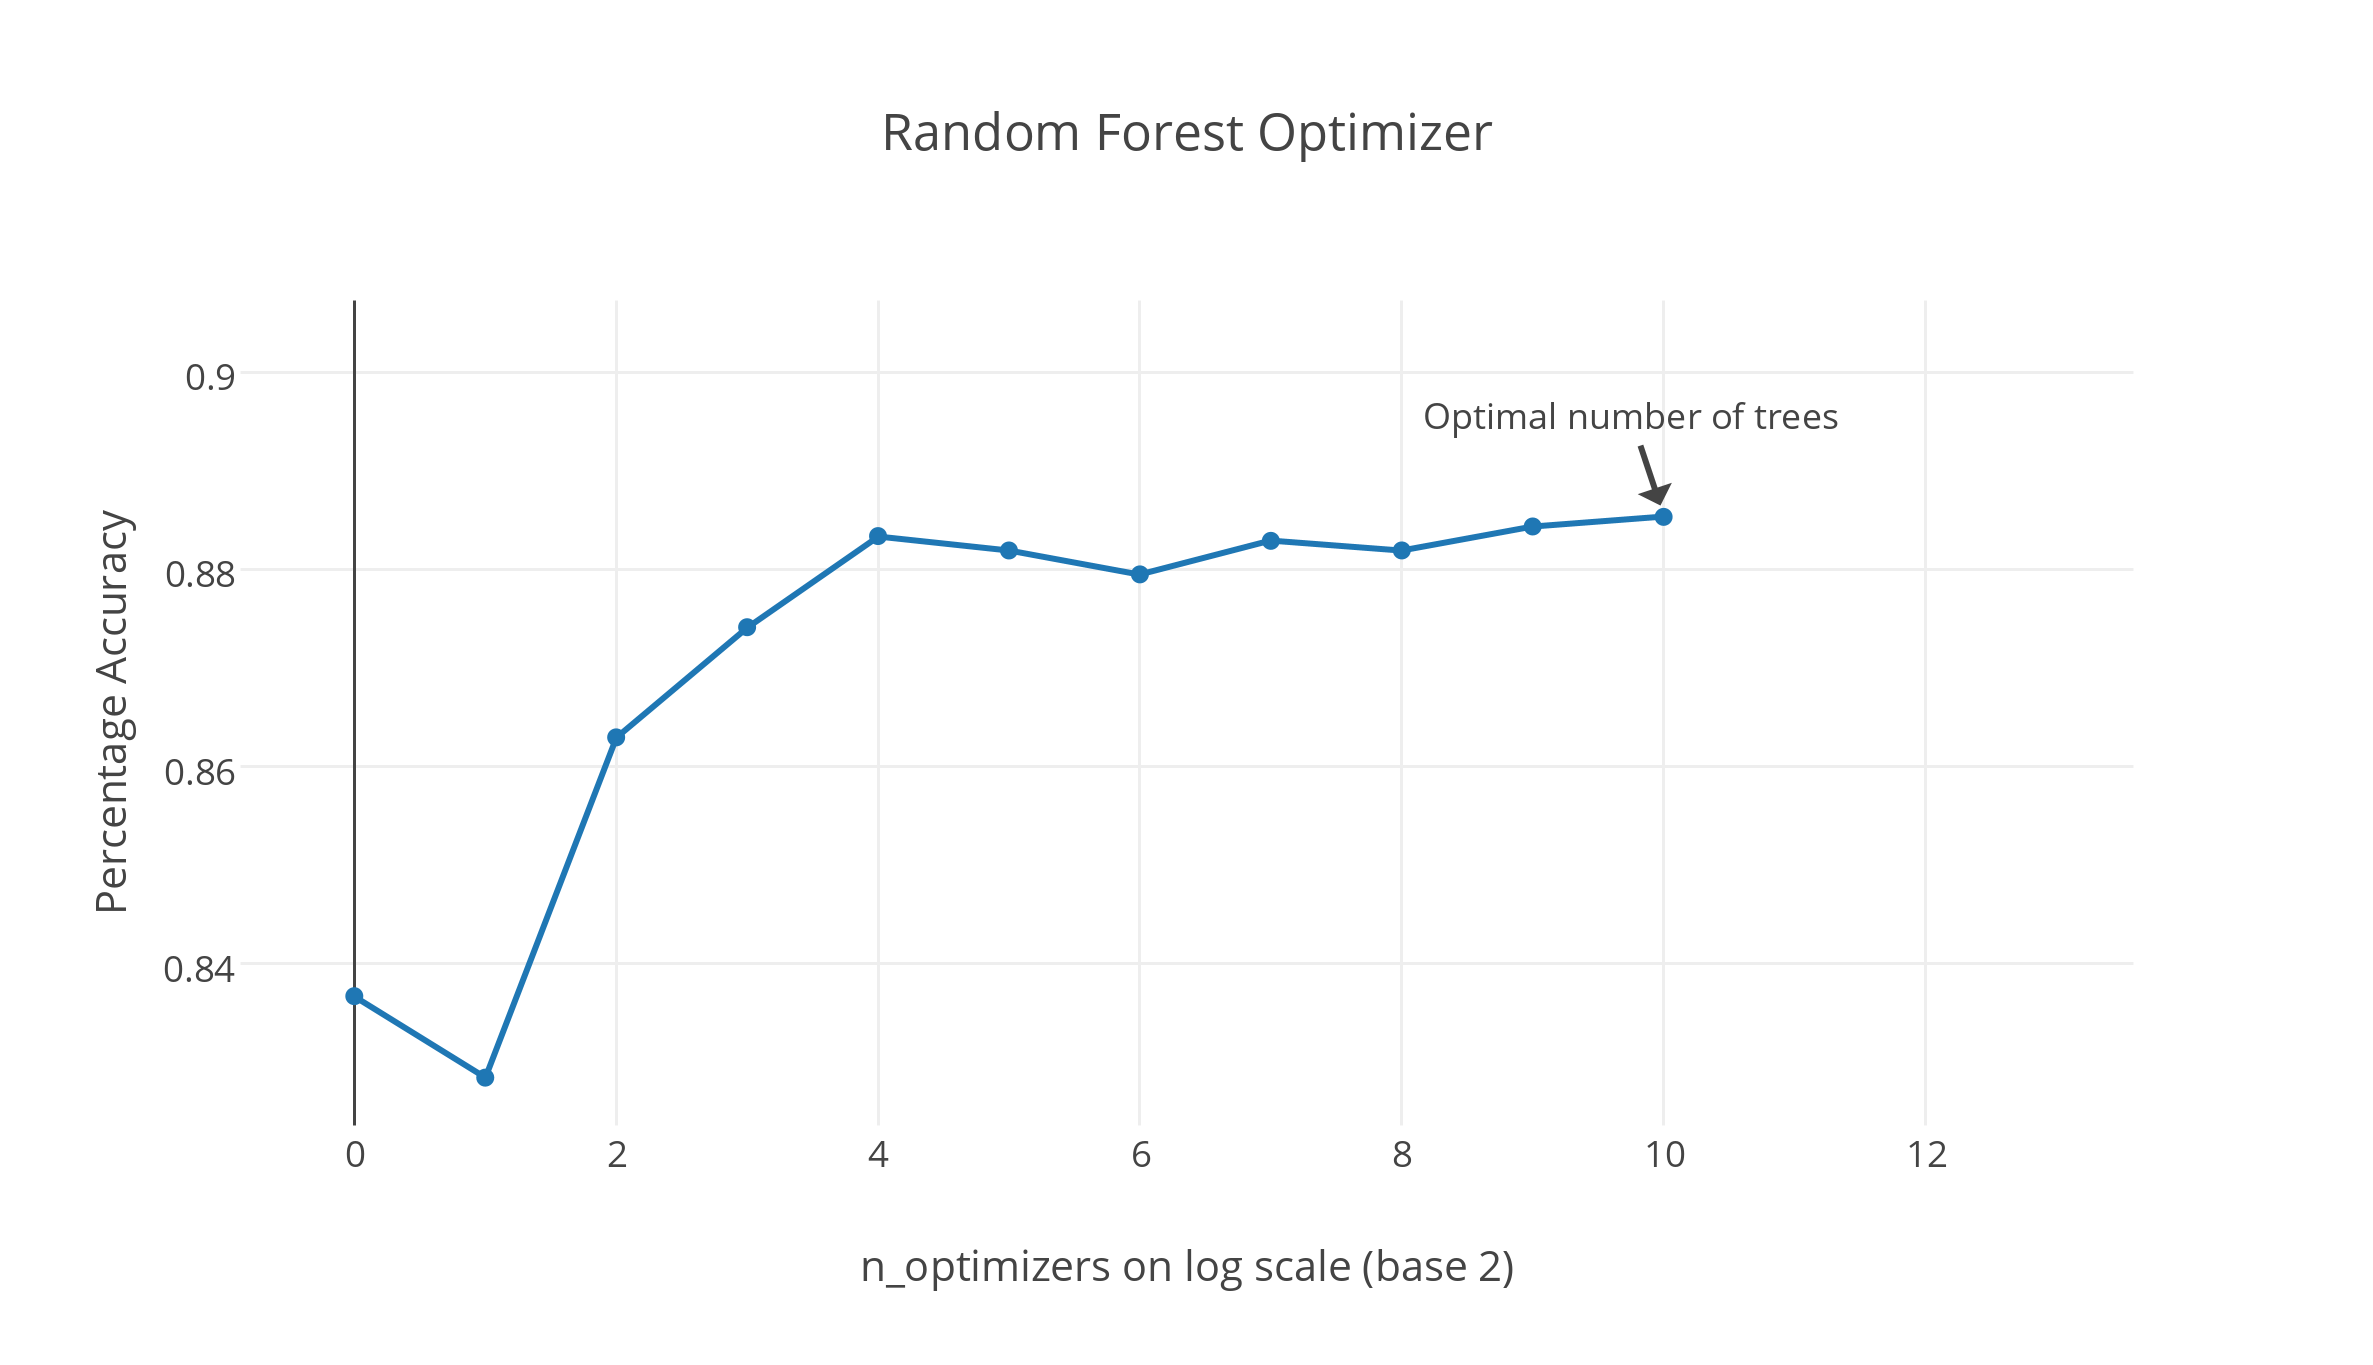
\includegraphics[scale=0.5]{random_forest_optimizer.png}
\caption{The graph showing how prediction accuracy from cross-validation changes with parameter n-estimators in the random forest classifier. The classifier generally works better for larger number of trees, but improvement in results are not significant after reaching 1024 trees.}
\label{fig:random_forest_optimizer}
\end{figure}

% Support Vector Machine
\subsection{Support Vector Machine}
Support vector machines make use of kernel functions to provide a new efficient way of separating non-linear functions. The potential upshots of using support vector machine methods is that there are well-researched theoretical guarantees about their performance, are not affected by local minima and do not suffer from the curse of dimensionality. The main idea behind SVMs are to maximize the margins between the decision boundary and the points that are hardest to classify, i.e. data points that lie closest to the decision surface, the set of which we call support vectors. In a J-dimensional feature space, the linear decision boundary is given by:
$$w^T\phi(x) + b = 0$$
The orthogonal distance from a point $\phi(x)$ to the decision boundary in space is given by:
$$\phi(x) = \phi(x)_{\perp} + r \frac{w}{|| w ||_2}$$
Solving for $r$, we get
$$r = \frac{w^T\phi(x) + b}{||w||_2} = \frac{f(x,w,b)}{||w||_2}$$
Let $t_n \in \{-1,1\}$ such that $t_n \cdot f(x_n,w,b) \ge 0$ when $x_n$ is correctly classified and $t_n \cdot f(x_n,w,b) \le 0$ when $x_n$ is wrongly classified, then the parameters that maximize the total margin over all data points are found by:
$$w^*, b^* = \argmax_{w,b} \frac{1}{||w||_2} \min_{n \in \{1,2,...,N\}} \{ t_n \cdot (w^T\phi(x_n) + b) \}$$
This is the optimization problem that SVMs try to solve. This can be reduced to a quadratic programming problem with a simple scaling trick.\\
\\
We attempted using sklearn's SVC and SGDClassifier models to see if they yielded better results according to our cross-validation. Optimization was conducted by changing important hyper-parameters including type of kernel (linear, poly, rbf or sigmoid) and penalty parameter C of error term. However, results obtained were routinely less satisfactory than those obtained with random forests.

% k-Nearest Neighbors
\subsection{k-Nearest Neighbors}

On the last practical we had some success with a k-Nearest Neighbors approach, so we decided that it was worth exploring for this problem as well. To get a benchmark, we first tried the simplest thing possible, which was using the Euclidean distance between test and training points as our similarity metric, and simply using the most common label among a point's k nearest neighbors as our prediction for that point with no regularization based on magnitude of distance. Table \ref{tab:knn_no_reg} shows the mean accuracy of these predictions of 20 random validation sets comprising of $\frac{1}{4}$ of the training data for various values of k.\

\begin{table}[h!]
\centering
\begin{tabular}{l|l}
k   & No regularization \\\hline\hline
1   & 0.840             \\
3   & 0.824             \\
5   & 0.826             \\
7   & 0.831             \\
12  & 0.824             \\
20  & 0.809             \\
30  & 0.806             \\
100 & 0.744            
\end{tabular}
\caption{Average Accuracy for unregularized predictions on 20 randomized validation sets}
\label{tab:knn_no_reg}
\end{table}
\noindent
But not all neighbors are created equal! Consider a the following basic example, where we t had $k=5$ and a given datum in the test set had the following 5 (distance, neighbor's class) points: (.2, 1), (.6, 1), (50, 2), (100, 2), (1000,2). While more of the point's nearest neighbors have class 2, the nieghbors in class 1 are MUCH more similar to point we are trying to classify. To help mitigate such this problem, we developed the following scheme to take the magnitude of distances into account: for each of the k nearest neighbors, we give $\frac{1}{\varepsilon + D_i}$ "points" to that neighbor's class (where $D_i$ is the distance between that neighbor and the point we wish to classify, and $\varepsilon$ is a weighting paramer), and predict the class with the highest score. Table \ref{tab:cross_validation_original} shows the mean accuracy for predictions on 20 random validation sets over different k and $\varepsilon$ pairs. As we can see there is a significant improvement in prediction accuracy on average, and an extra two percent accuracy with the best k,$\varepsilon$ pair over the optimal k from Table \ref{tab:knn_no_reg}\\\\
\noindent
Improvements for our KNN approach did not stop here. Noticing that file sizes had large variance, we decided to try scaling our features that were "counts" of certain system calls by dividing by filesize in MB. A quick look at Table \ref{tab:cross_validation_scaled} shows that in general this lead to small increases in average prediction accuracy for most k, $\varepsilon$ pairs. In doing this it occured to us that since we were only dividing count features by filesize, binary features were being given more weight under our distance metric. To adjust for this, we ended up standardizing our features by dividing everything by its standard deviation. Looking at table \ref{tab:cross_validation_normalized}, it's easy to see that this was a good call, as prediction accuracy improved accross by board by a couple percent, with several k, $\varepsilon$ pairs above 87 percent accuracy, and one as high as 88 percent! (It should be noted that we tried this scaling by filesize and normalizing by sd on our features before runing random forests as well, but without any improvement, likely because the random forest approach ends up weighting features itself). Unfortunately while these improvements did carry over to the test set (increase between submissions 8 and 10 in Figure \ref{fig:scores_large}, our best KNN submission only got around 75 percent accuracy. This disparity is likely due to the different makeup of the Test and Training data (see Figure \ref{fig:pie_chart_train} and Figure \ref{fig:pie_chart_test}), as well our distance metric not taking into account the fact that some features are just more useful/important than others for classifying malware. More about this in the k-Nearest Neighbors Revisited section in Further Development.


% Features
\subsection{Feature Selection}
\noindent Feature Selection is an important part of machine learning - some would argue, it is the most important part. We are not part of that ``some''. While we found that feature selection improved our score, it is interesting to note that despite including more and more features, our best performing model, the random forest, never improved by any significant margin. In fact, we had our performance consistently work than our first iteration of feature extraction.\\

\begin{figure}
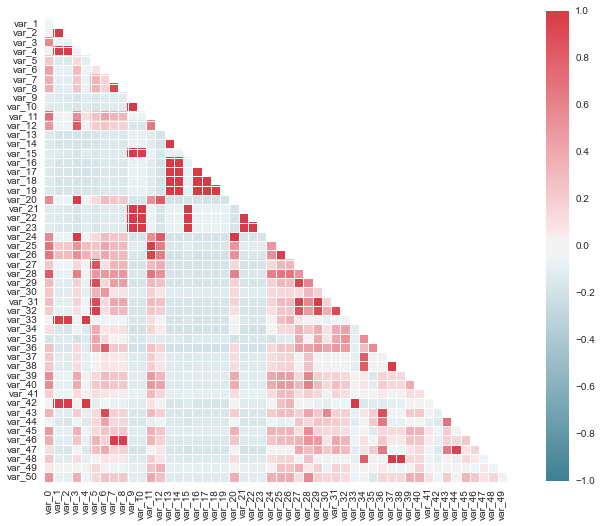
\includegraphics[scale=0.4]{covariance}
\caption{The correlation plot between the first 50 features selected in our generative model. While we did not remove features with high-correlation, the plot indicates an interesting trend - either features were highly and positively correlated, or not-correlated at all.}
\label{fig:correlation_plot}
\end{figure}

\noindent To begin, we were provided with sample code which extracted three important features from each file:
\begin{enumerate}
\item First system call. For each XML file, we also extracted the first system call. While this is a single feature for a single executable, the extraction can actually lead to over 3000 features (imagine each XML file has a different initial system call). This feature was binary - you either used X as your first system call, or you did not.

\item Last system call. Similar to the above. The feature is also binary and adds up to 3000 features. However, combined with the above, we found that these two function actually added only a total of 136 new features to our training set. This implies a high correlation between initial and final calls across multiple executable files, which intuitively makes sense. We also hypothesize that these are the highly correlated features in Figure \ref{fig:correlation_plot}.

\item Number of System Calls. Each XML file contains a single all\_sections tag between which all remaining tags are system calls. The provided code counted the number of tags between all\_section, thereby counting the number of system calls performed by a single executable.

\item System call counts. As an extension of total number of system calls, we also decided to count the number of calls made to each system call. This added approximately $\ell$ features, where $\ell$ is the total number of unique system calls used by our entire datasets. In practice, this number was relatively small, around 2500. 

\item Longest Sequence of System Calls. This feature scanned input XML files and found the longest sequence of equivalent system calls, creating a feature per sequence. In the worst case, this creates approximately 3000 new features for our entire training set. This was our first idea behind capturing the ``structure'' of the execution diagram. To visualize this, note that every execution of a program creates a type of dependency graph, as shown in \ref{fig:dependency_diagram}, and we attempted to capture some of the structure of this graph through this ``longest sequence'' feature.

\item n-grams (in terms of system calls). As an extension to the above, in order to capture further structure information on the execution trace of the provided programs, we decided to implement a polymorphic feature function which allowed us to extract the count of sequence of length $k$ from a particular XML trace file. In other words, for each sequence of $k$ system calls we encountered during our processing of the datums, we would create a new feature for that unique sequence. Then value for this feature then became the number of times that particular sequence occurred within each XML file. In general, this algorithm is theoretically inefficient. Given $\ell$ unique system calls, there are up to $\ell!$ possible sequences (order matters). We know that:
\begin{align*}
	\ell! \geq \left(\frac{\ell}{2}\right)^{\left(\frac{\ell}{2}\right)} \tag{$\forall \ell > 0$}
\end{align*}
thereby providing us with an exponential lower-bound. However, in practice, we found this was not the case. Sequences seemed to repeat themselves quite often, and not all possible sequences of length $\ell$ were present. In fact, even after extracting all $6$-grams (in terms of tags) from our training set, we still had only 100,000 features per datum. 

\item URL Connections. From some simple analysis and shallow browsing of the XML files within our training set, we noted that suspicious files tended to connect to suspicious websites. Therefore, we added a feature which attempted to capture this information. For each tag which contained the word "server", "address", or "url", we created a new feature with the value of the tag and added this to our set of features. 

\item Bag of Words (not actually used in submissions due to large number of features generated). Surprisingly enough, at the start of the problem set, we figured it might be possible to simply treat the XML files as text files and extract information from them that way. In particular, following the example of the previous top-scorer on Kaggle last practical, we decided to attempt a bag of words feature which would simply split the input XML file in bags of words and count each occurrence. This led to the creation of an unmanageable number of features, and was therefore abandoned moving forward. another reason for the abandonment was the fat that it led to our worst prediction yet on Kaggle. We were unable to determine the root cause of the problem, but as can be seen in Figure \ref{fig:scores}, our second generative model failed expectaculary. Simply added bag of words to this model. It's possible that the failure was due to a bug in the code rather than the 
\end{enumerate}

\noindent In general, we developed three approaches to feature selection. The first approach focused on simply extracting count information from the XML files (such as total number of system calls, etc.). The second approach involved extracting information on the structure of the program execution itself, through the extraction of repeated sequences. The last approach was simply extracting features that we intuitively believed to be important based on some simple analysis of the files within the training data set (such as connections to servers). However, all of these approaches proved to cause little difference in our finals scores, as we can see from Figure \ref{fig:scores_large}. As soon as we added unique system call counts and switched to a Random Forest Classifier, our scores improved significantly. After that point, the only other improvement came from the addition of n-grams, but it was relatively small, and due to the nature of random forests, it is difficult to draw a conclusion as to its actual effect on the accuracy of the predictions. 


\begin{figure}[h!]
\centering
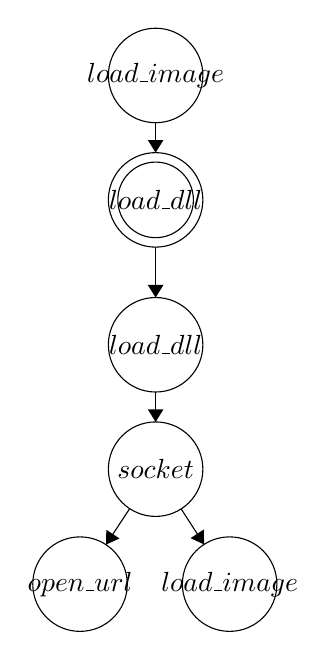
\begin{tikzpicture}[scale=0.2]
\tikzstyle{every node}+=[inner sep=0pt]
\draw [black] (38.2,-13.8) circle (3);
\draw (38.2,-13.8) node {$load\_dll$};
\draw [black] (38.2,-13.8) circle (2.4);
\draw [black] (38.2,-23) circle (3);
\draw (38.2,-23) node {$load\_dll$};
\draw [black] (38.2,-30.9) circle (3);
\draw (38.2,-30.9) node {$socket$};
\draw [black] (33.4,-38.2) circle (3);
\draw (33.4,-38.2) node {$open\_url$};
\draw [black] (42.9,-38.2) circle (3);
\draw (42.9,-38.2) node {$load\_image$};
\draw [black] (38.2,-5.9) circle (3);
\draw (38.2,-5.9) node {$load\_image$};
\draw [black] (38.2,-16.8) -- (38.2,-20);
\fill [black] (38.2,-20) -- (38.7,-19.2) -- (37.7,-19.2);
\draw [black] (38.2,-26) -- (38.2,-27.9);
\fill [black] (38.2,-27.9) -- (38.7,-27.1) -- (37.7,-27.1);
\draw [black] (36.55,-33.41) -- (35.05,-35.69);
\fill [black] (35.05,-35.69) -- (35.91,-35.3) -- (35.07,-34.75);
\draw [black] (39.82,-33.42) -- (41.28,-35.68);
\fill [black] (41.28,-35.68) -- (41.26,-34.73) -- (40.42,-35.28);
\draw [black] (38.2,-8.9) -- (38.2,-10.8);
\fill [black] (38.2,-10.8) -- (38.7,-10) -- (37.7,-10);
\end{tikzpicture}
\caption{Sample DAG showing possible execution path of a program. For each program, we determined the structure of this graph correlated well with the class of the program. Intuitively, the way a program behaves is determined more by the sequence of class it makes}
\label{fig:dependency_diagram}
\end{figure}


\section{Results and Discussion}
In this section, we discuss the results obtained from the different models attempted and features extracted. In general, the discussion is divided into each specific model, however, we found that multiple results applied to different models (such as improving feature selection), and so such discussion has been moved to the section ``Feature Selection and Other''.\\
\\
\noindent To begin, we take a look at the change over time of our Kaggle scores, graphically depicted in Figure \ref{fig:scores}.

\begin{figure}[h!]
 \centering
 \includegraphics[scale=0.2]{privatepublic_kaggle_scores}
 \caption{Both private and Public Kaggle Scores over time. During development, only public scores were available. Notable features include: (1) bug in feature extraction, (2) consistent under-performance on private tests, (3) consistent under-performance of  KKN as compared to Random Forest, and (4) Lack of significant improvement after reaching maximum.}
 \label{fig:scores}
\end{figure}

\subsection{Generative Model}
\noindent As discussed in Methods, the generative approach proved to be rather ineffective due to the inability to include a sizable number of features caused by the small $N_k$ for $k= 9$. In Figure \ref{fig:correlation_plot} we can see the correlation between our selected features, which totaled 3289 features (we therefore only show a correlation plot between a random subset of 50). Interestingly enough, it seems that only minority of the features were strongly correlated, and no features were very negatively correlated. Our hypothesis for this is that, typically, system calls in a system are not redundant and relatively atomic. Therefore, a higher count of one system call tends to correlate with larger file size (due to the atomic nature of system calls), which correlates with higher other system calls. In the other direction, system calls don't really tend to replace each other - they're not redundant. Therefore, there's no real reason to find a negative correlation between particular system calls.\\
\\
\noindent Given the above results, we were surprised to find that our system performed relatively poorly when using additional features provided by bag of words. It's possible that our code for extracting words from an XML file is buggy, but taking a look at it below, it appears correct and our tests indicate its correctness (code can be found in Section \ref{sec:code}). Our only possible alternative is that with so many features (over 100,000), the inverse covariance matrix for all of our classes was singular, forcing the utilization of the Moore-Penrose pseudo inverse which hindered the predictability of our model.

\subsection{Random Forest}
\noindent The best performing method turned out to be random forests. We've already described their internal workings in the methods section, as well as our process for optimizing the meta-parameters, therefore this section's man focus is discussing the final results of our most optimal method. In our most optimal method, we used all features discussed above except bag-of-words. For n-grams, we only consider up to 3-grams as the computational and memory requirements of higher n-grams prevented us from training our model.

\begin{figure}[h!]
	\centering
    \includegraphics[scale=0.33]{pie_training_data}
    \caption{Pie chart of the malware class distributions in the training data set}
    \label{fig:pie_chart_train}
\end{figure}

\begin{figure}[h!]
	\centering
    \includegraphics[scale=0.33]{pie_testing_data}
    \caption{Pie chart of the malware class distributions in the training data set}
    \label{fig:pie_chart_test}
\end{figure}

\noindent We begin by discussing the results of our model in terms of the distribution of the classes on the data set. As shown by Figure \ref{fig:pie_chart_train} and Figure \ref{fig:pie_chart_test}, the distributions of malware between our training set and our test set are very different. Simply looking at the Poison class, where our training set only had $2$ datums, we immediately see a large difference. The test set contained about $10$ times more (20) such classifications. It's difficult to see how an algorithm could train on a universe where the Poison class is so rare and still be expected to perform well in one where it is not, but this highlights the need for models to generalize well, rather than just predict well. In general, the testing set simply had far more datums which were classified as malware than the training set. 

\begin{figure}[h!]
	\centering
    \includegraphics[scale=0.33]{pie_scored_data}
    \caption{Pie chart of the malware class distributions as predicted by optimal algorithm.}
    \label{fig:pie_chart_scored}
\end{figure}

\noindent In Figure \ref{fig:pie_chart_scored}, we see the predicted distribution for the test data based on our random forest model. It's evident that the under-representation of virus classes affected our predictions. However, focusing on the Posion malware, we're encouraged to note the increase from $0.68$ to $3.0$. Given only two data points, the random forest model was able to successfully classify a good number of Poison malware, and the under classification is expected. In general, the random forest model seems to have generalized well as the predicted distribution reflects both the effects of the training data as well as the expected effects of the test data.

\section{Further Development}
\subsection{Neural Networks (possibly)}
\noindent While we do not expect neural nets to perform any better in this problem than our random forest solution \footnote{\href{http://www.cs.cornell.edu/~caruana/ctp/ct.papers/caruana.icml06.pdf}{An Empirical Comparison of Supervised Learning Algorithms}}, a future step in this research could possibly be the exploration of optimal parameters for neural nets in order to maximize accuracy. 

\subsection{k-Nearest Neighbors Revisited}
As mentioned earlier, the biggest issue with out k-Nearest Neighbors approach was that it did not take feature importance into account. By using the Euclidean distance between points as our distance metric, we are giving each feature equal weight, when in reality this is not what we want to do. The ideal scenario would be to heavily weight features that have high between-class variance, but low inter-class variance. One way we could have found such features would have been by using a multiclass generalization of Fisher's Linear Disciminant, as described in Bishop 4.1.6. Additionally we would have liked to implement similar attribute wieghted KNN methods discussed in \href{https://books.google.com/books?id=qm_SBQAAQBAJ&pg=PA165&lpg=PA165&dq=classification+find+features+with+low+intra+class+variance+high+inter+class+variance&source=bl&ots=CRE2ln-JwE&sig=wViY6RYVFFhI4gx8Ai8p939FFn0&hl=en&sa=X&ei=esj4VMjNDMflsATBqYG4CA&ved=0CCAQ6AEwAA#v=onepage&q=classification\%20find\%20features\%20with\%20low\%20intra\%20class\%20variance\%20high\%20inter\%20class\%20variance&f=false}{Data Classification: Algorithms and Applications (2014)}. Given the decent performance of KNN with a naive Euclidean distance metric, we are interested in seeing how well this metod would have performed, though due to time contraints were unable to pursue it further.

\subsection{Feature Selection Revisited}
One possible idea for improving feature selection is to generalize our n-gram approach to system calls, and instead, actually compute the DAG for each XML file. We can then run an algorithm over the data set for each class which allows us to find common substructures of the graph. In the general case, this problem appears to be NP-hard, since even the fastest algorithm for a simpler problem of finding the most common string in a set of strings appears to take exponential time. However, a paper \footnote{\href{http://web.cs.ucdavis.edu/~gusfield/cs224f11/commonsubstrings.pdf}{Common Substring of More than Two Strings}} we found suggests it's solvable much more quickly. We did not find the time to understand or implement the algorithm, or to generalize it for DAGs. We believe the structure of the program's execution history a very important feature for classification, if not the most important.

\section{Conclusion}
The problem of classifying malware given its execution trace is difficult. However, after attempting multiple different models and extracting many different features from the provided XML files, we found random forest to perform the best. It incorporates re-normalization to avoid over-fitting and selects the best features. Empirically, it is not only simple to implement, but also performs well. Disappointingly, feature extraction proved less successful. After extracting basic counts along with some simple program execution information using n-grams, we discovered our random forest model performed only minimally better than with other simpler features. In fact, due to the random nature of the classifications the random forest model provides, we often times  found a decrease in performance despite an increase in the number of features provided per datum. We conclude that a random forest classifier is likely to perform well on the problem of malware classification, and with improved features, in particular features about the execution structure of the program in question, it might possible to determine classes of malware with high accuracy. However, we recommend using a larger data set than that provided, and if possible, one which is more similar to what is likely to be  found in the wild. The difference between our testing data set and training data set appears to have guaranteed a somewhat low accuracy score for any model.

\onecolumn

\subsection{Large Figures and Tables}
Below, we provide access to larger versions of our figures as well as detailed tables referenced in the text.

\begin{table}[h!]
\begin{center}
    \begin{tabular}{ | p{1cm} | p{2cm} | p{1cm} | p{1cm} | p{1cm} |}
    \hline
    Virus Name \# & Virus Type & \% in Train & \% in Test & \% Predicted \\ \hline
    0 & Agent & 3.69 & 7.40 & 3.92 \\ \hline
    1 & AutoRun & 1.62 & 1.65 & 1.34 \\ \hline
    2 & FraudLoad & 1.20 & 1.54 & 1.61 \\ \hline
    3 & FraudPack & 1.03 & 1.37 & 0.99 \\ \hline 
    4 & Hupigon & 1.33 & 1.81& 1.18 \\ \hline
    5 & Krap & 1.26 & 1.65 & 2.01 \\ \hline
    6 & Lipler & 1.72 & 1.21 & 1.56 \\ \hline 
    7 & Magania & 1.33 & 1.59 & 1.66 \\ \hline 
    8 & None & 52.14 & 41.39 & 46.64\\ \hline
    9 & Poison & 0.68 & 4.22 & 2.95\\ \hline
    10 & Swizzor & 17.56 & 16.83 & 18.45\\ \hline
    11 & Tdss & 1.04 & 1.86  &1.64 \\ \hline
    12 & VB & 12.18 & 13.10 & 13.24 \\ \hline
    13 & Virut & 1.91 & 3.56 & 1.93\\ \hline 
   	14 & Zbot & 1.30 & .82 & 0.86 \\ \hline 
    \end{tabular}
    \caption{Classes and their distributions in the training data and the testing data. As can be seen, the testing data must have a different distribution than the training data, posing an additional challenge to the problem of accurately predicting the classes for each test datum.}
    \label{tab:virus_classes}
\end{center}
\end{table}


\begin{table}[h!]
\centering
\begin{tabular}{l|lllllll}
K   & 0.001 & 0.01  & 0.05  & 0.1   & 0.2   & 1     & 10\\\hline\hline % inserts single horizontal line
1   & 0.836 & 0.843 & 0.837 & 0.837 & 0.835 & 0.838 & 0.841 \\
3   & 0.850 & 0.846 & 0.847 & 0.845 & 0.847 & 0.846 & 0.845 \\
5   & 0.855 & 0.857 & 0.851 & 0.854 & 0.849 & 0.855 & 0.852 \\
7   & 0.857 & 0.856 & 0.852 & 0.856 & 0.855 & 0.853 & 0.853 \\
12  & 0.856 & 0.855 & 0.850 & 0.851 & 0.851 & 0.853 & 0.846 \\
20  & 0.853 & 0.852 & 0.852 & 0.849 & 0.848 & 0.852 & 0.844 \\
30  & 0.848 & 0.851 & 0.849 & 0.845 & 0.849 & 0.846 & 0.837 \\
100 & 0.830 & 0.828 & 0.829 & 0.828 & 0.824 & 0.826 & 0.806
\end{tabular}
\caption{Table of Validation results for different values of K and epsilon on original data.}
\label{tab:cross_validation_original}
\end{table}



\begin{table}[h!]
\centering

\begin{tabular}{l|lllllll}
K   & 0.001 & 0.01  & 0.05  & 0.1   & 0.2   & 1     & 10\\\hline\hline % inserts single horizontal line
1   & 0.847 & 0.844 & 0.845 & 0.839 & 0.840 & 0.847 & 0.846 \\
3   & 0.849 & 0.844 & 0.851 & 0.849 & 0.851 & 0.848 & 0.846 \\
5   & 0.855 & 0.853 & 0.853 & 0.853 & 0.858 & 0.848 & 0.842 \\
7   & 0.855 & 0.859 & 0.859 & 0.860 & 0.856 & 0.843 & 0.839 \\
12  & 0.861 & 0.856 & 0.854 & 0.852 & 0.855 & 0.840 & 0.835 \\
20  & 0.853 & 0.851 & 0.851 & 0.848 & 0.843 & 0.829 & 0.824 \\
30  & 0.849 & 0.847 & 0.846 & 0.838 & 0.834 & 0.819 & 0.810 \\
100 & 0.825 & 0.823 & 0.819 & 0.812 & 0.798 & 0.779 & 0.756
\end{tabular}
\caption{Table of Validation results for different values of K and epsilon on unnormalized scaled data.}
\label{tab:cross_validation_scaled}

\end{table}


\begin{table}[h!]
\centering

\begin{tabular}{l|lllllll}
K   & 0.001 & 0.01  & 0.05  & 0.1   & 0.2   & 1     & 10\\\hline\hline % inserts single horizontal line
1   & 0.858 & 0.861 & 0.864 & 0.863 & 0.861 & 0.862 & 0.861 \\
3   & 0.871 & 0.866 & 0.873 & 0.868 & 0.869 & 0.870 & 0.863 \\
5   & 0.869 & 0.871 & 0.874 & 0.871 & 0.876 & 0.871 & 0.858 \\
7   & 0.874 & 0.877 & 0.874 & 0.873 & 0.868 & 0.871 & 0.860 \\
12  & 0.875 & 0.874 & 0.874 & 0.880 & 0.876 & 0.870 & 0.861 \\
20  & 0.875 & 0.874 & 0.873 & 0.874 & 0.875 & 0.868 & 0.853 \\
30  & 0.867 & 0.867 & 0.873 & 0.872 & 0.868 & 0.862 & 0.835 \\
100 & 0.838 & 0.837 & 0.835 & 0.833 & 0.827 & 0.800 & 0.761
\end{tabular}
\caption{Table of Validation results for different values of K and epsilon on normalized scaled data.}
\label{tab:cross_validation_normalized}
\end{table}

\begin{figure}[h!]
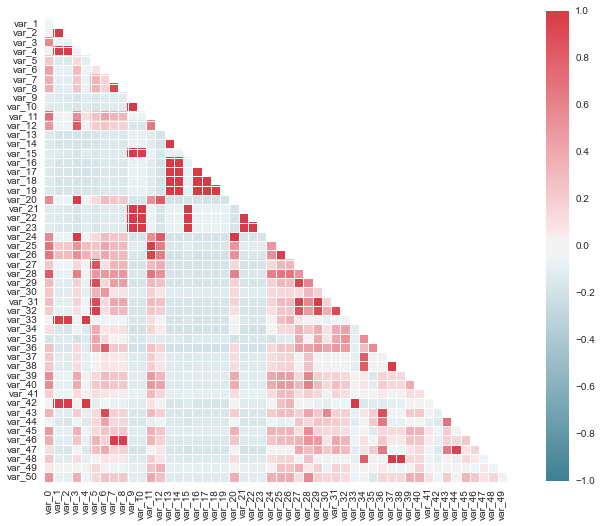
\includegraphics[scale=0.9]{covariance}
\caption{Large version of correlation plot.}
\label{fig:correlation_plot_large}
\end{figure}

\begin{figure}[h!]
	\centering
	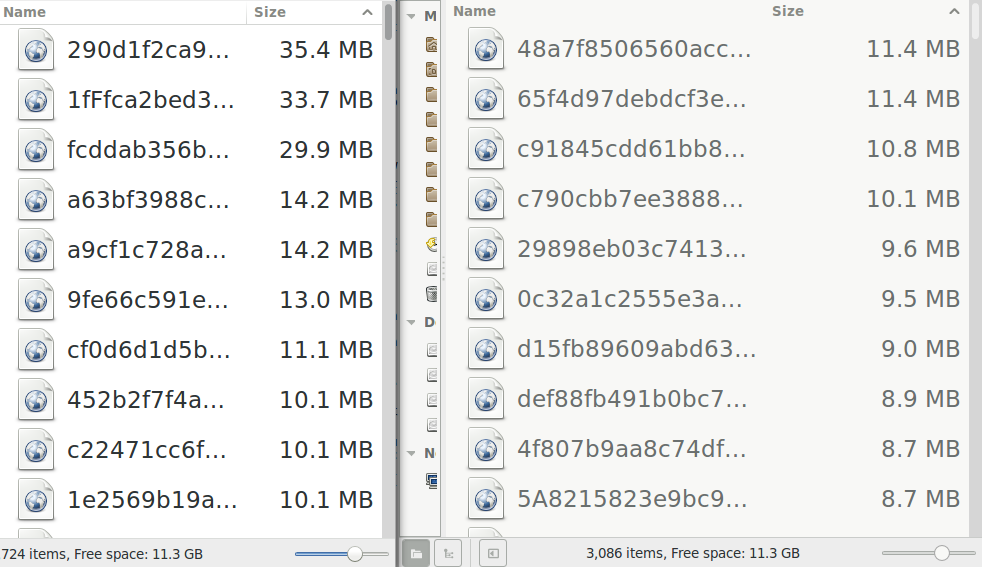
\includegraphics[scale=0.4]{file_size}
    \caption{Large version of file-size screen shot.}
    \label{fig:file_size_large}
\end{figure}

\begin{figure}[h!]
 \centering
 \includegraphics[scale=0.5]{privatepublic_kaggle_scores}
 \caption{Both private and public Kaggle Scores over time. During development, only public scores were available. Notable features include: (1) bug in feature extraction, (2) consistent under-performance on private tests, (3) consistent under-performance of  KKN as compared to Random Forest, and (4) lack of significant improvement after reaching maximum.}
 \label{fig:scores_large}
\end{figure}

\begin{figure}[h!]
	\centering
    \includegraphics[scale=0.7]{pie_training_data}
    \caption{Pie chart of the malware class distributions in the training data set}
    \label{fig:pie_chart_train_large}
\end{figure}

\begin{figure}[h!]
	\centering
    \includegraphics[scale=0.7]{pie_testing_data}
    \caption{Pie chart of the malware class distributions in the test data set as deduced after submission deadline from the Kaggle competition. The distribution is over the private test cases, not the public tests (thereby explaining the discrepancy in the ``None'' class.}
    \label{fig:pie_chart_test_large}
\end{figure}

\begin{figure}[h!]
	\centering
    \includegraphics[scale=0.7]{pie_scored_data}
    \caption{Pie chart of the malware class distributions as predicted by optimal algorithm.}
    \label{fig:pie_chart_scored_large}
\end{figure}

\pagebreak
\clearpage
\section{Code}
 \label{sec:code}
\begin{lstlisting}[language=Python]
def bag_of_words_feat(tree, frequency=False, count=True, subset=10):
    # we want to extract words using regular expressions
    import re
    
    root = tree.getroot()
    text = ET.tostring(root)
    split_text = re.findall(r"[\w']+", text)
    cv = sklearn.feature_extraction.text.CountVectorizer(split_text)
    cv.fit_transform(split_text)
    
    # count words in counter (positive and negative)
    vocab = Counter({key: cv.vocabulary_[key] for key in cv.vocabulary_.keys() 
    	if cv.vocabulary_[key]}) if count else {}
    vocabNeg = Counter({key: -value for key,value in vocab.items()})
    
    # subset accordingly
    vocabMost = {key: value for key,value in vocab.most_common(subset)} 
    	if subset > 0 else vocab
    vocabLeast = {key + "_least": -value for key,value in vocabNeg.most_common(subset)} 
    	if subset > 0 else vocab
    
    # count frequencies
    totalMFreq = sum(vocabMost.values())
    totalLFreq = sum(vocabLeast.values())
    
    # frequency dictionaries
    freq_dict = {key + "_freq" :(value/totalMFreq) for key,value in vocabMost.items()} 
    	if frequency else {}
    least_freq_dict = {key + "_freq" : (value/totalLFreq) for key, value in vocabLeast.items()} 
    	if frequency else {}
    
    return dict(vocabMost.items() + vocabLeast.items() + freq_dict.items() +
    	least_freq_dict.items())
\end{lstlisting}

\end{document}